\documentclass[preview]{standalone}

\usepackage{amsmath}
\usepackage{amssymb}
\usepackage{parskip}
\usepackage{fullpage}
\usepackage{hyperref}
\usepackage{tikz}
\usepackage{stellar}

\usetikzlibrary{angles,quotes}

\hypersetup{
    colorlinks=true,
    linkcolor=black,
    urlcolor=blue,
    pdftitle={Physical Rendering},
    pdfpagemode=FullScreen,
}

\begin{document}

\title{Physical Rendering}
\id{physicalrendering}
\genpage

\section{Measurements}

\subsection{Radiant Flux}

\begin{snippet}{radiant-flux-definition}
\sdefinition{Radiant Flux}{
    The \textit{radiant flux} (or power) \(\Phi\) is the total amount of energy passing
    through a surface per second and is measured in \([W]\) (Watts) as \(\frac{J}{s}\).
}
\end{snippet}

\subsection{Irradiance}

\begin{snippet}{irradiance-definition}
\sdefinition{Irradiance}{
    The \textit{irradiance} \(E\) is the measurements of the radiant flux per \textit{unit area}
    and is measured in \([W]{[M]}^{-2}\) as \(\frac{\Phi}{m^2}\).
}
\end{snippet}

\subsection{Radiance}

\begin{snippet}{radiance-definition}
\sdefinition{Radiance}{
    The radiance \(L\) is the irradiance per unit solid angle (steradian) and is
    measured in \([W]{[M]}^{-2}{[sr]}^{-1}\) as \(\frac{E}{sr}\).
}
\end{snippet}

\section{Geometry}

\subsection{Fundamental vectors}

\begin{snippet}{fundamental-vectors-illustration}
% tikz picture
\begin{center}
    \begin{tikzpicture}
        \draw (-4,0) -- (4, 0);
        \draw (0,0) coordinate (a) -- (-3, 3) coordinate (b);
        \draw[->] (a) -- (0, 3) coordinate (c);
        \draw[->] (a) -- (3, 3) coordinate (d);

        \node[below] at (a) {\(x\)};
        \node[right] at (d) {\({\hat{V}}^t\)};
        \node[left] at (b) {\(\hat{V}\)};
        \node[left] at (c) {\(\hat{N}\)};
        \node[right] at (c) {\(\hat{L},\hat{R}\)};

        \pic["\({\theta}_r\)", draw=black, -, angle eccentricity=1.2, angle radius=1cm] {angle=d--a--c};
        \pic["\({\theta}_i\)", draw=black, -, angle eccentricity=1.2, angle radius=1cm] {angle=c--a--b};
    \end{tikzpicture}
\end{center}

\begin{itemize}
    \item \(\hat{V}\) direction torwards the camera
    \item \(\hat{N}\) surface normal
    \item \(\hat{L}\) vector pointing torward the light source
    \item \(\hat{R}\) reflected ray direction
    \item \({\theta}_i, {\theta}_r\) incident and reflected angles
\end{itemize}

The reflected ray is given by \(\hat{R}=\hat{L}-2\hat{N}(\hat{L}\cdot\hat{N})\).
\end{snippet}

\subsection{Light attenuation}

\begin{snippet}{light-attenuation}
The amount of radiance on a point is given by
\[
    \Phi \left(\hat{L} \cdot \hat{N}\right) = \Phi \cdot \cos(\alpha)
\]
where \(\alpha\) is the angle between the two vectors.
\\
This means that if the light source is perfectly above the point, then
there is no light attenuation \((\alpha = 0)\).
\end{snippet}

\section{Materials}

\subsection{Types of materials}

\begin{snippet}{types-of-material-reflections}
Different materials reflect incoming light to different directions and absord different amounts of it.

\begin{center}
    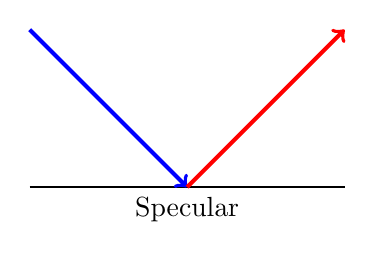
\begin{tikzpicture}[scale=2]
        % surface
        \draw[line width=0.25mm] (-1,0) -- (1, 0);

        % ray in
        \draw[->][line width=0.5mm, color=blue] (-1,1) -- (0, 0);

        % rays out
        \draw[->][line width=0.5mm, color=red] (0,0) -- (1, 1);

        % label
        \node[below] at (0,0) {Specular};
    \end{tikzpicture}
    \qquad
    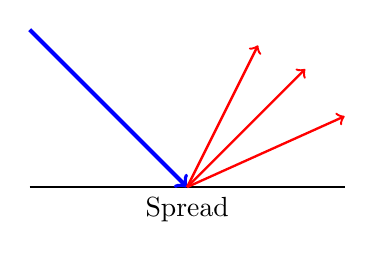
\begin{tikzpicture}[scale=2]
        % surface
        \draw[line width=0.25mm] (-1,0) -- (1, 0);

        % ray in
        \draw[->][line width=0.5mm, color=blue] (-1,1) -- (0, 0);
        
        % rays out
        \draw[->][line width=0.3mm, color=red] (0,0) -- (0.75, 0.75);
        \draw[->][line width=0.3mm, color=red] (0,0) -- (0.45, 0.9);
        \draw[->][line width=0.3mm, color=red] (0,0) -- (1, 0.45);

        % label
        \node[below] at (0,0) {Spread};
    \end{tikzpicture}
    \qquad
    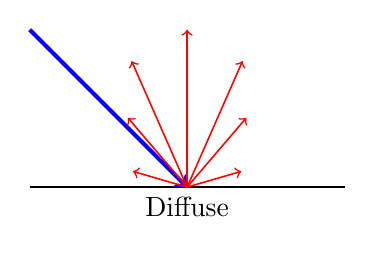
\begin{tikzpicture}[scale=2]
        % surface
        \draw[line width=0.25mm] (-1,0) -- (1, 0);

        % ray in
        \draw[->][line width=0.5mm, color=blue] (-1,1) -- (0, 0);
        
        % rays out
        \draw[->][line width=0.2mm, color=red] (0,0) -- (0.376, 0.44);
        \draw[->][line width=0.2mm, color=red] (0,0) -- (-0.376, 0.44);
        \draw[->][line width=0.2mm, color=red] (0,0) -- (0.352, 0.8);
        \draw[->][line width=0.2mm, color=red] (0,0) -- (-0.352, 0.8);
        \draw[->][line width=0.2mm, color=red] (0,0) -- (0.344, 0.1);
        \draw[->][line width=0.2mm, color=red] (0,0) -- (-0.344, 0.1);
        \draw[->][line width=0.2mm, color=red] (0,0) -- (0, 1);

        % label
        \node[below] at (0,0) {Diffuse};
    \end{tikzpicture}
\end{center}
\end{snippet}

\subsection{Bidirectional reflectance distribution function}

\begin{snippet}{brdf-definition}
\sdefinition{Bidirectional reflectance distribution function}{
    The \textit{BRDF function} (Bidirectional reflectance distribution function) is a probability distribution
    for the amount of light reflected in a certain direction.
    \[
        f_r(\hat{w}, x, \hat{w}^\prime)
    \]
    where
    \begin{itemize}
        \item \(\hat{w}\) incoming ray direction
        \item \(x\) point of collision
        \item \(\hat{w}^\prime\) outgoing ray direction
    \end{itemize}
    The function follows the following properties:
    \begin{enumerate}
        \item \textbf{Helmholtz-reciprocity}:
        \(
            \forall \hat{w},x,\hat{w}^\prime, \quad f_r(\hat{w}, x, \hat{w}^\prime) = f_r(\hat{w}^\prime, x, \hat{w})
        \)
        \item \textbf{positivity}:
        \(
            \forall \hat{w},x,\hat{w}^\prime, \quad f_r(\hat{w}, x, \hat{w}^\prime) \geq 0
        \)
        \item \textbf{energy conversation}:
        \[
            \int_\Omega f_r(\hat{w}, x, \hat{w}^\prime) \cos \theta \, d\hat{w}^\prime \leq 1
        \]
    \end{enumerate}
    where \(\Omega\) encloses the scene (usually a hemisphere).
}
\end{snippet}

\subsection{Bidirectional transmittance distribution function}

\begin{snippet}{btdf}
If a material can also transfer light through itself, we use the BTDF function
(Bidirectional transmittance distribution function).
\end{snippet}

\subsection{Bidirectional scattering distribution function}

\begin{snippet}{bsdf}
We use the BSDF or BxDF (Bidirectional scattering distribution function)
to generalize both the BTDF and BRDF.
\end{snippet}

\section{Rendering equation}

\begin{snippet}{rendering-equation-definition}
\sdefinition{Rendering Equation}{
    The \textit{rendering equation} tells us how much radiance is exiting a \textit{surface point}
    in a given direction. Note that objects may also be emitting light.
    \[
        \textit{Light exiting point} = \textit{Material emitted light} + \textit{Reflected incoming light}
    \]
    Formally,
    \[
        L_o(x, \vec{\omega})
        =L_e(x, \vec{\omega})
        +\int_\Omega L_i(x,\vec{\omega})f_r(\vec{\omega}, x, \vec{\omega}^\prime)
        \cos \theta d\vec{\omega}^\prime
    \]
    
    \begin{itemize}
        \item \(L_o\) outgoing radiance from point \(x\) in the direction \(\vec{\omega}\)
        \item \(L_e\) emitted radiance from point \(x\) in the direction \(\vec{\omega}\) by the object itself
        \item \(\Omega\) scene
        \item \(L_i\) incoming radiance to point \(x\) from the direction \(\vec{\omega}\)
        \item \(f_r\) BRDF
        \item \(\cos \theta\) light attenuation
    \end{itemize}
    
    This value is difficult to compute. For each point, the light at that point
    depends on the incoming radiance of every other point, which also depends on the first point.
    This integral is infinite-dimensional because of the infinite bounces.
}
\end{snippet}

\section{Phong reflection model}

\begin{snippet}{phone-reflection-model}
The phong reflection model is an approximation
to the rendering equation.
\end{snippet}

\subsection{Simplified ambient BRDF model}

\begin{snippet}{simplified-ambient-brdf-model}
\[
    I=k_a I_a
\]
\begin{itemize}
    \item \(k_a\) ambient coefficient of an object (base color)
    \item \(I_a\) ambient intensity of the scene/light sources
\end{itemize}
\end{snippet}

\subsection{Simplified diffuse BRDF model}

\begin{snippet}{simplified-diffuse-brdf-model}
\[
    I_d=k_d (\vec{L} \cdot \vec{N})
\]

\begin{itemize}
    \item \(k_d\) diffuse coefficient of an object
    \item \(\vec{L}\) vector pointing to the light vector
    \item \(\vec{N}\) surface normal
\end{itemize}
\end{snippet}

\subsection{Simplified specular BRDF model}

\begin{snippet}{simplified-specular-brdf-model}
\[
    I_s=k_s {(\vec{V} \cdot \vec{R})}^n
\]

\begin{itemize}
    \item \(k_s\) specular coefficient of an object
    \item \(\vec{V}\) direction towards the camera
    \item \(\vec{R}\) reflected direction of the light ray
    \item \(\vec{n}\) shininess factor
\end{itemize}
\end{snippet}

\subsection{Result}

\begin{snippet}{phone-result-illustration}
The sum of the phone simplified models
gives a good approximation to the rendering equation.

\begin{figure}[h]
    \centering
    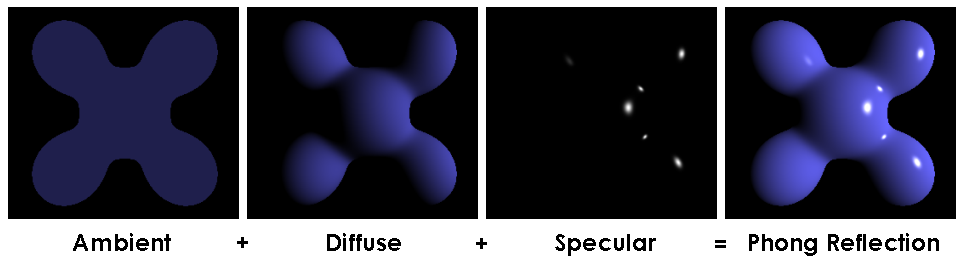
\includegraphics[width=0.8\textwidth]{resources/phong.png}
\end{figure}
% In the shader I do return surfaceColor * (spec + dif);

The diffuse and ambient values must be computed for each light in the scene.
It is sufficient to consider only the light rays that hit the camera, meaning
we can trace rays from the camera to the point, and assume that they're reflections
from the light.

Note that the specular intensity cannot be precomputed as it is dependant
on the camera position.

\end{snippet}

\section{Reflection and refraction}

\begin{snippet}{reflection-refraction-illustration}
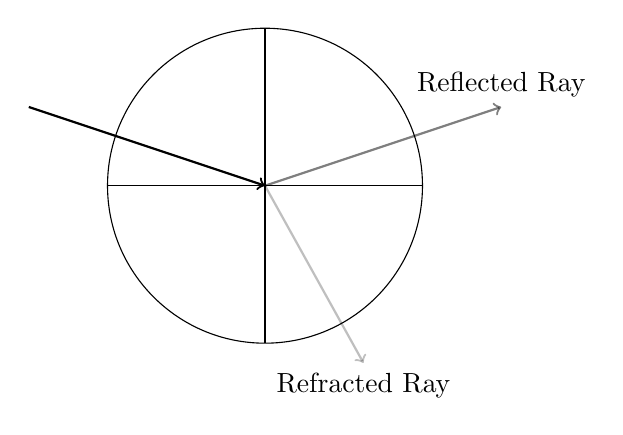
\begin{tikzpicture}
    \draw (0,0) circle [radius=2cm];
    
    % Incoming ray
    \draw[->, thick] (-3,1) -- (0,0);

    % Reflected ray
    \draw[->, thick, opacity=0.5] (0,0) -- (3,1)
        node[above, opacity=1] {Reflected Ray};

    % Refracted ray
    \draw[->, thick, opacity=0.25] (0,0) -- (1.25,-2.25)
        node[below, opacity=1] {Refracted Ray};
    
    % Incident angle
    %\draw [dashed] (-3,0) arc [start angle=180, end angle=140, radius=3cm];
    %\node at (-2.5, 0.5) {$\theta_i$};
    
    \draw[-] (0,-2) -- (0,2);
    \draw[-] (-2,0) -- (2,0);
    
\end{tikzpicture}
\end{snippet}

ASSETS TO USE


The Fresnel Equation

\[
    R_s(\theta) =
        \left|
            \frac
            {
                n_1\cos \theta - n_2 \sqrt{1-{\left(\frac{n_1}{n_2}\sin \theta\right)}^2}
            }
            {
                n_1\cos \theta + n_2 \sqrt{1-{\left(\frac{n_1}{n_2}\sin \theta\right)}^2}
            }
        \right|
\]

Snell's law

\[
    \frac{\sin \theta_1}{\sin \theta_2}
    = \frac{V_1}{V_2}
    = \frac{n_2}{n_1}
\]

\end{document}
